\section{State of the Art}
Grob betrachtet können verlustbehaftete Kompressionen in drei Teilschritte aufgeteilt werden: Transformation, Quantisierung und Entropie Kodierung. Die Abbildung \ref{state:aufbau} zeigt eine vereinfachte Abfolge. Die Inputdaten werden zuerst duch ein oder mehrere Verfahren transformiert. So transformieren, dass in der Quantisierung unwichtige Informationen gelöscht werden können. Hier geschieht der Datenverlust. Danach werden die Daten Entropie Kodiert, was wieder verlustfrei ist. Unterschiedliche Verfahren für jeden Teilschritt. Meist auch mehrere Transformationen, oder Transformation Quantisierung Transformation Quantisierung.\\
\begin{figure}[!htbp]
	\center
	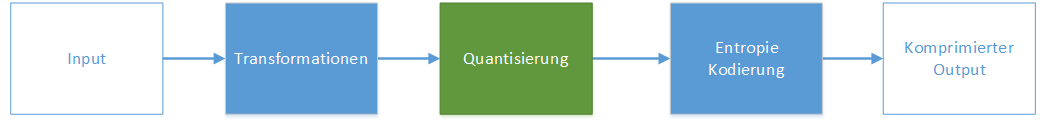
\includegraphics[width=0.8\textwidth,height=6cm,keepaspectratio]{./pictures/state/aufbau.png}
	\caption{Typische Teilschritte einer Kompression}
	\label{state:aufbau}
\end{figure}
Folgend werden Kompressionsverfahren oder typische Algorithmen für einen Teilschritt beschrieben.

\subsection{JPEG/JFIF Kompression}
Weit verbreitete Bild
YCbCr, DCT, Quantisierung, Entropie Kodierung.

\subsection{3d Mesh Kompression}
In der Computergrafik müssen alle Gegenstände und Akteure in der virtuellen Welt modelliert werden. So wird ein Mensch eine Menge von Dreiecken, das Mesh, modelliert. Jeder Punkt eines Dreieck kann zusätzliche Informationen gespeichert haben wie Texturkoordinaten, Farbe oder Oberflächen-Normalen. Je nach Anwendungsfall kann ein Modell aus ein paar hundert oder mehreren hunderttausend Dreiecken bestehen. Um diese Datenmenge zu verkleinern versuchen Formate wie OpenCTM \cite{website:openctm} die Datenmenge verlustfrei oder verlustbehaftet zu komprimieren.\\
wie funktioniert es\\

wie es verwendet werden könnte

\subsection{PointCloud Kompression}
Industrie Lasersampling
Bild pointcloud
Grosse Punktmenge, welche im 3d Raum komprimiert werden soll.
verlustfrei/ Verlustbehaftet
Je nach Implementation können zu jedem Punkt zusatzinfos gespeichert werden wie Farbe/Normalen etc, darüber könnte die Information, zu welcher Linie ein Punkt gehört, gespeichert werden.

\subsection{Signal Approximation}
Messtechnik von Medizin bis Fotografie, überall wo man ein Signal über Zeit hat
Versucht ein Signal durch eine Folge von Funktionen zu approximieren.

Gute Approximation kommt mit wenigen Funktionen aus.
Verlustbehaftete Kompression, indem man mit einer begrenzten Anzahl

fourier, wavelet Compressed sensing, Spline Approximation

\subsection{Entropie Kodierung}
Verlustfreie Komprimierung basierend auf Shannons coding theorem

 Arithmeic, Huffman
Dictionary Type: LZ77, Byte paoir encoding, RLE
